\section{Results}

In our experiments, we aim to answer the following questions:
\begin{enumerate}
    \vspace{-0.5em}
    \item How well does \agentname{} perform at achieving both text and visual goals in Minecraft?
    \vspace{-0.25em}
    \item How does our method scale with more data?
    \vspace{-0.25em}
    \item What choices are important for the performance of our method?
\end{enumerate}

\subsection{Training Setup}

We base our implementation off of the official VPT codebase\footnote{ \href{https://github.com/openai/Video-Pre-Training}{https://github.com/openai/Video-Pre-Training}}. The main \agentname{} agent is trained using Pytorch \citep{pytorch} distributed data parallel on four A40 GPUs for 160M frames, or just under three epochs of our gameplay dataset. Hyperparameters are selected to match those in \citet{baker2022vpt} with the exception of learning rate, which we set to 4e-5. Our models are optimized using AdamW \citep{adamw}. See \autoref{table:model_hparams} for a full list of hyperparameters.

\subsection{Performance on Textual and Visual Goals}
\label{sec:exp_perf}

\begin{figure}
    \centering
    \begin{subfigure}{0.49\textwidth}
        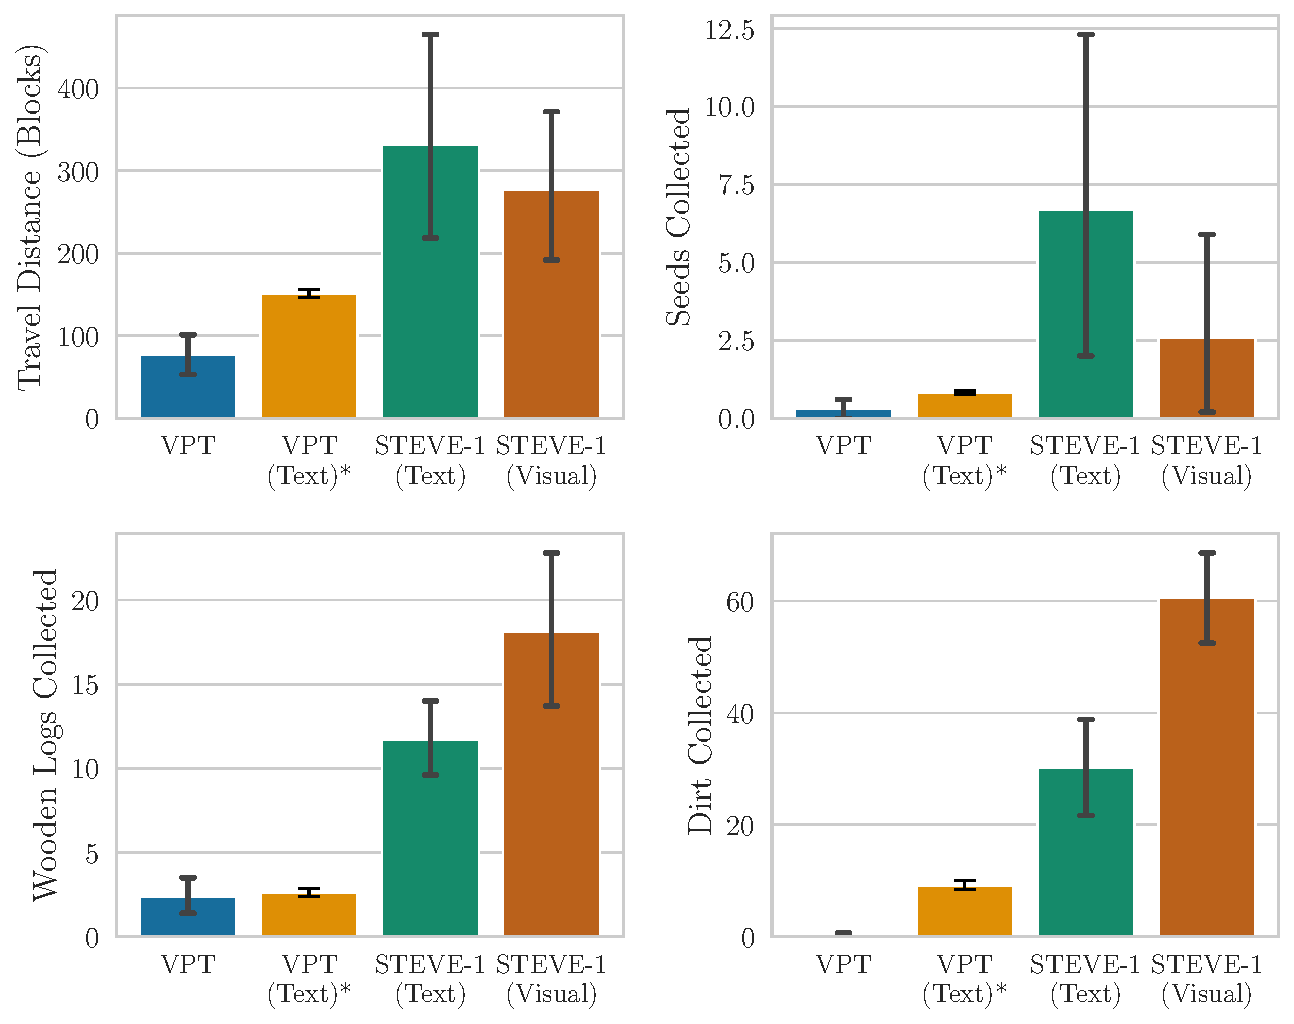
\includegraphics[width=\textwidth]{figures/4.2_final_perf_camera_ready.pdf} 
        \caption{Programmatic Evaluation}
        \label{fig:final_perf_prog}
    \end{subfigure}
    \begin{subfigure}{0.49\textwidth}
        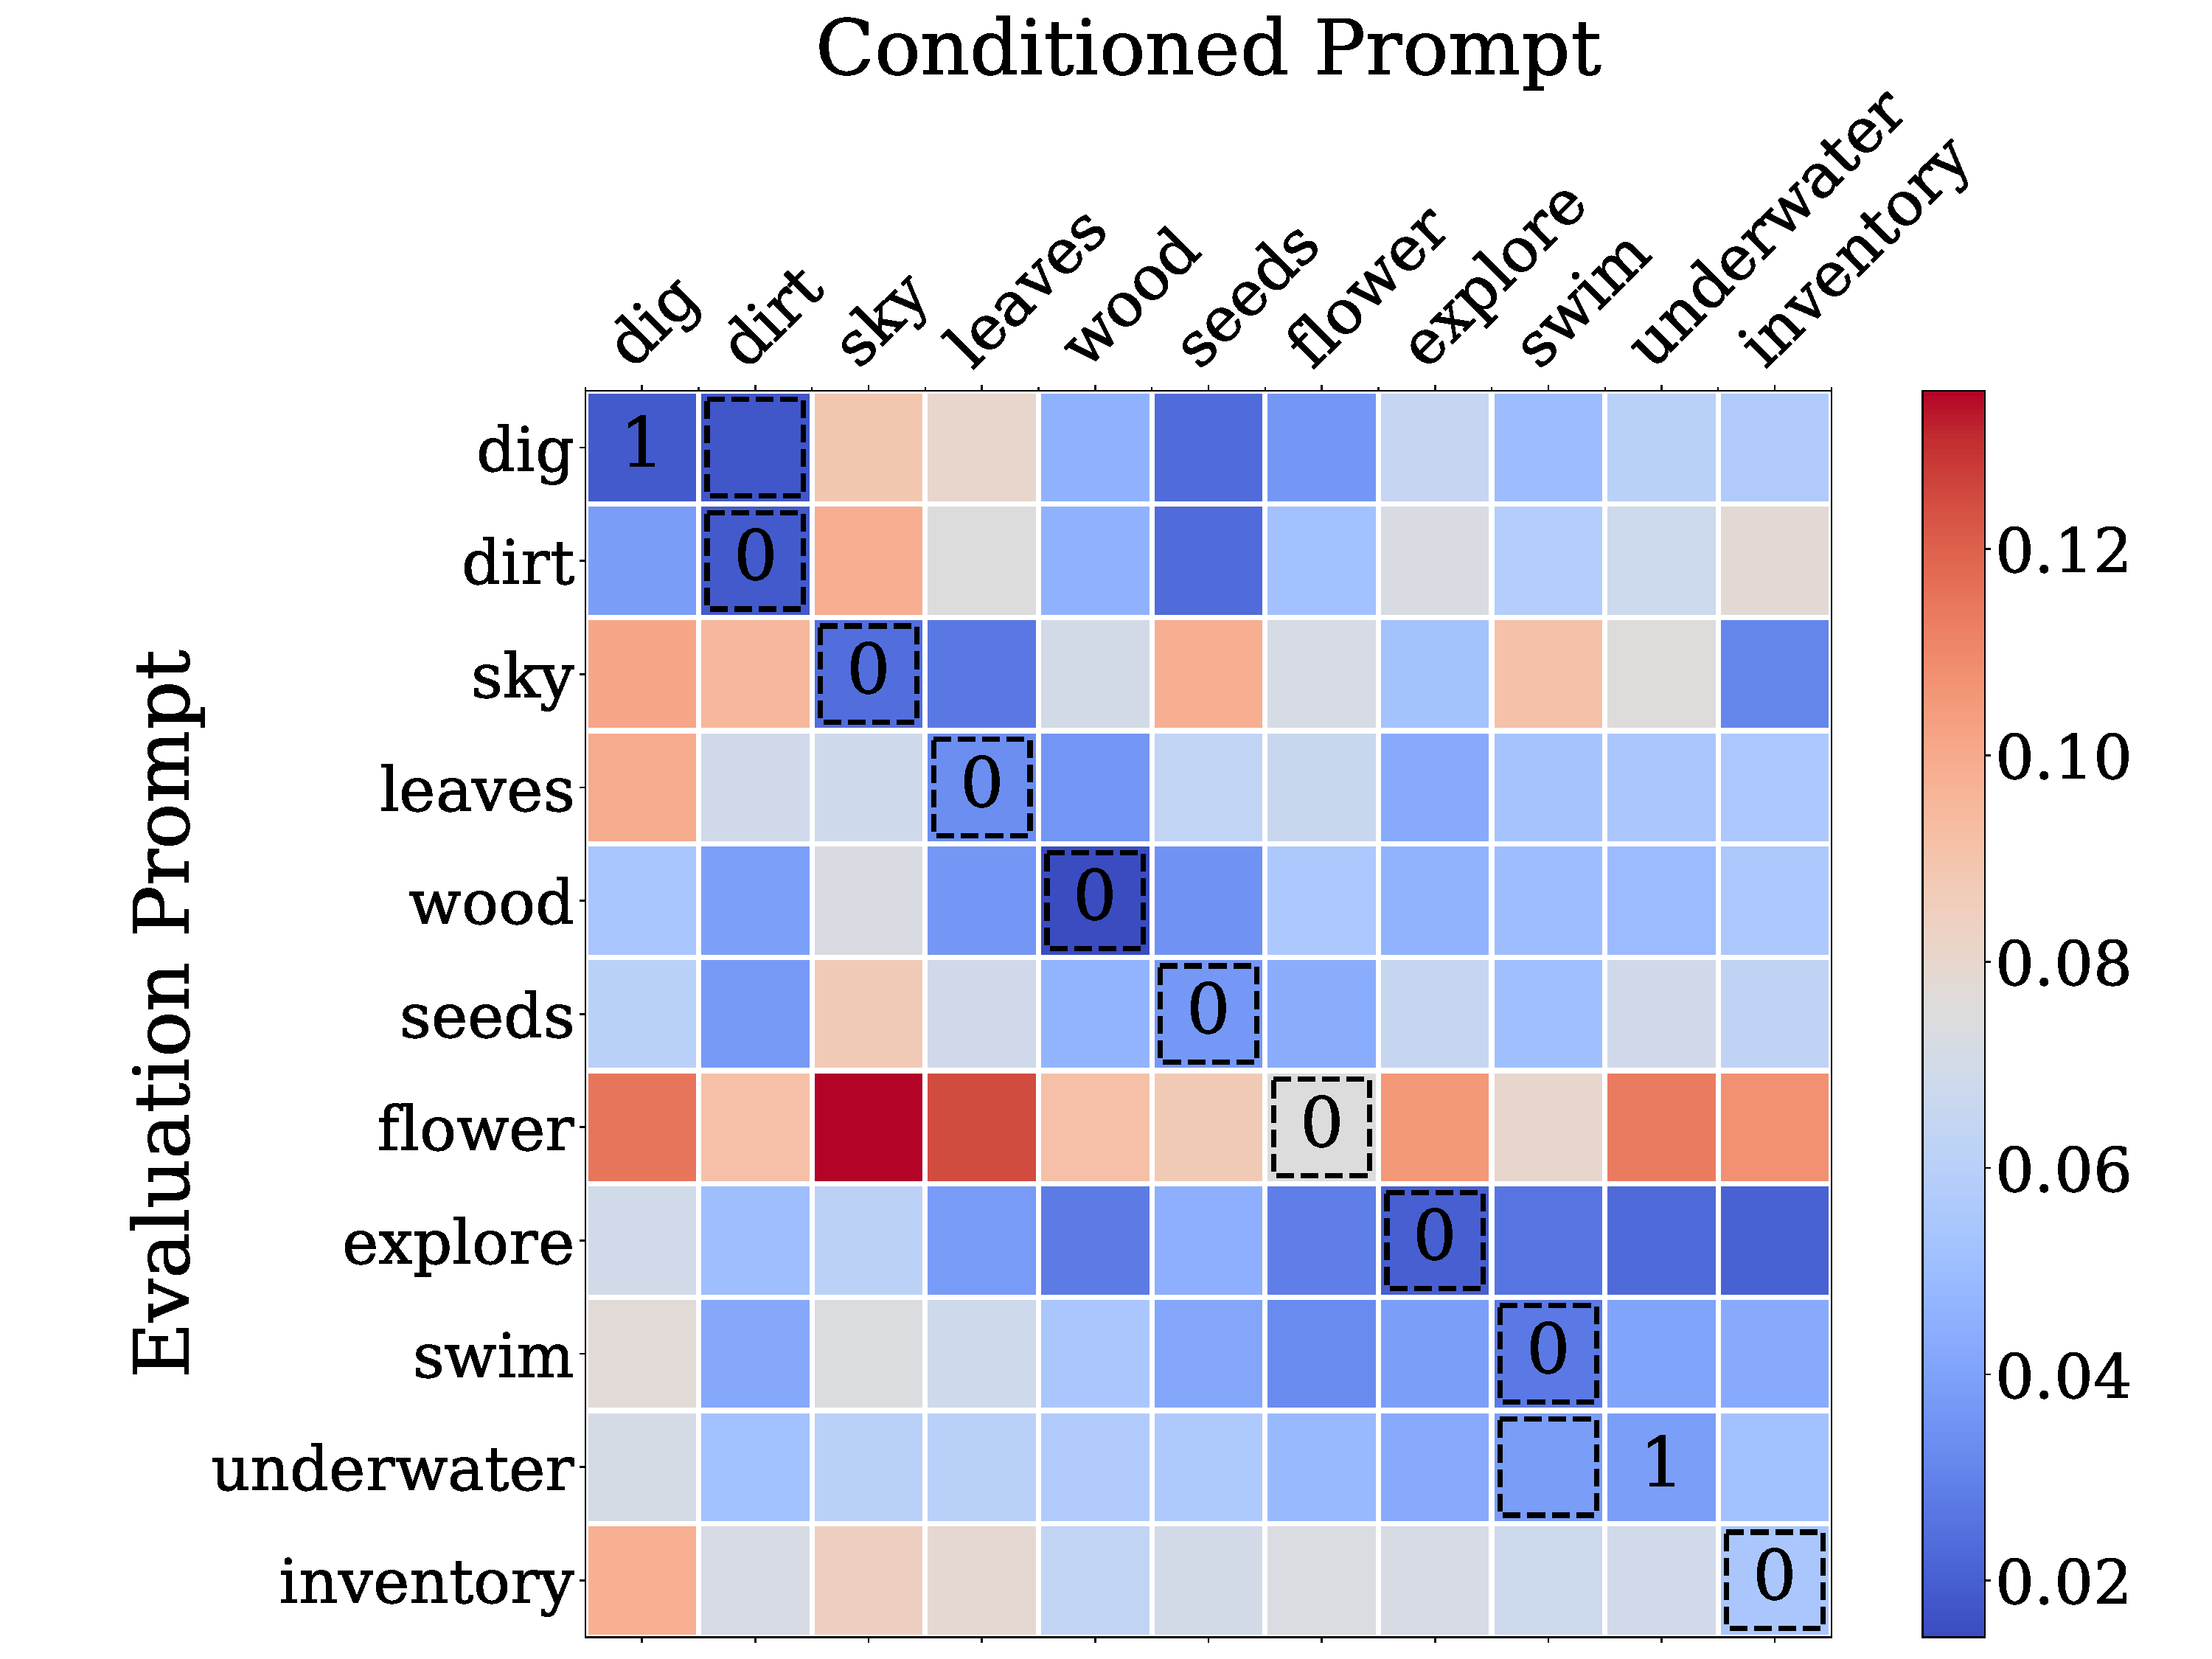
\includegraphics[width=\textwidth]{figures/4.2_final_perf_mineclip.pdf}
        \vspace{0.1em}
        \caption{MineCLIP Evaluation}
        \label{fig:final_perf_mineclip}
    \end{subfigure}
    \caption{
    \textbf{Left:} 
    In our programmatic evaluations, \agentname{} performed far better than the unconditional VPT agent \texttt{early-game-2x} and the text-conditioned VPT agent when prompted appropriately. The asterisk * in the ``VPT (Text)*'' indicates that this result was taken from Appendix I in \citep{baker2022vpt}, which had twice the episode length compared to our setting. On some tasks, visual outperforms text-based prompting, creating a gap that can likely be bridged through better prompt engineering. 
    \textbf{Right:} 
    Across our 11 MineCLIP evaluation tasks, \agentname{} achieves the shortest distance between the episode and the MineCLIP goal embedding when prompted appropriately except for in two cases, where it mixes up digging and dirt and swimming and going underwater. This shows the strong general performance of \agentname{} across a wide variety of short-horizon tasks. The dashed box marks the minimum element along the row, and the diagonal number signifies the diagonal element's rank (0 means it is the minimum row element). See \autoref{fig:apdx_visual_goals} for sample frames from each of the 11 visual goals and  \autoref{fig:success_rate_matrix} for a success-rate version of this matrix.
    }
    \label{fig:final_perf}
    \vspace{-1em}
\end{figure}

Due to the hierarchical nature of our model, we can evaluate the performance of our agent at achieving either text or visual goals simply by choosing whether to use the prior to condition on text or bypass the prior and condition on a MineCLIP video embedding directly. We first tested our model on a set of 11 tasks that are achievable within the first 2.5 minutes of gameplay and which do not require multiple steps to complete (e.g., chop a tree or dig a hole, but not build a house). A complete list of the tasks and prompts we used for evaluation can be found in \autoref{tab:apdx_text_prompt} in the appendix. To select visual goals for testing each of the evaluation tasks, we implemented a tool that searches through 10\% of our gameplay dataset by finding the closest 16-frame videos to a given text prompt. We then manually selected a 16-frame video that clearly demonstrates the task being completed and use the corresponding MineCLIP video embedding as the goal embedding for that task. Screenshots of these visual goals can be found in \autoref{fig:apdx_visual_goals} in the appendix.

In \autoref{fig:final_perf}, we compare the performance of our text and visual-conditioned agents with the unconditional VPT agent and text-conditioned VPT agent (from Appendix I in \citep{baker2022vpt}) across our programmatic tasks. We find that when given the relevant text instruction, \agentname{} collects \(75 \times\) more dirt, \(4.9 \times\) more wood, \(22 \times\) more seeds, and travels \(4.3 \times\) farther than the unconditional agent, and \agentname{} collects \(3.3 \times\) more dirt, \(4.4 \times\) more wood, \(8.1 \times\) more seeds, and travels \(2.2 \times\) farther than the text-conditioned VPT agent. This represents a significant improvement over the reported performance of text-conditioned VPT, which collects several times fewer resources despite having twice as long of an episode to do so. We also run an automatic evaluation using MineCLIP embedding distances by measuring the minimum distance of a goal embedding to any frame in the episode. As shown in \autoref{fig:final_perf_mineclip}, the distance between the goal and the episode is significantly lower when the agent is conditioned on the corresponding visual goal than otherwise. Full results for \agentname{} with both text and visual goals can be found in \Cref{appendix:additional_vis}.

In addition to our evaluations of \agentname{}, we also recorded several sample interactive sessions we had with the agent (controlling it in real-time by giving it written text instructions or specific visual goals). These sessions demonstrate \agentname{}'s ability to responsively follow instructions in real-time in a variety of situations. We believe that such use-cases, where humans give an agent natural instructions that it can follow to complete tasks, will become increasingly important and have practical uses in the creation of instructable assistants and virtual-world characters. These videos, as well as videos of our agent performing our evaluation tasks, can be found at \href{https://sites.google.com/view/steve-1}{https://sites.google.com/view/steve-1}.

\subsection{Prompt Chaining}
\label{sec:exp_chaining}
We also experiment with longer horizon tasks that require multiple steps, such as crafting and building. We explore two different prompting methods: directly prompting with the target goal, and a simple form of prompt chaining \citep{Chase2022, wei2022chain, dohan2022language} where the task is decomposed into several subtasks and the prompts are given sequentially for a fixed number of steps. We explore prompt chaining with visual goals for two tasks: 1) building a tower and 2) making wooden planks. When using prompt chaining, we first prompt \agentname{} to gather dirt before building a tower, and to gather wooden logs before crafting wooden planks. \autoref{fig:chaining} shows that directly prompting \agentname{} with the final tasks results in near-zero success rates. However, prompt chaining allows \agentname{} to build a tower 50\% of the time and craft wooden planks 70\% of the time. 
For the tower building task, \agentname{} immediately starts collecting dirt until the prompt switches, at which point its average height starts increasing rapidly and its dirt decreases as it builds a tower. Similarly, for the crafting wooden planks task, \agentname{} immediately starts collecting a large amount of wooden logs until the prompt switches and it rapidly converts these wooden logs into wooden planks (causing the amount of wooden logs in its inventory to immediately decrease and the number of wooden planks to increase as it crafts more). \autoref{fig:chaining} visualizes the average item counts and agent height for the prompt chaining episodes. See \autoref{fig:apdx_chaining_tower_episode_main} and  \autoref{fig:apdx_chaining_planks_episode_main} in the appendix for visualizations of specific prompt chaining episodes.

\begin{figure}
    \centering
    \begin{subfigure}{0.48\textwidth}
        \centering
        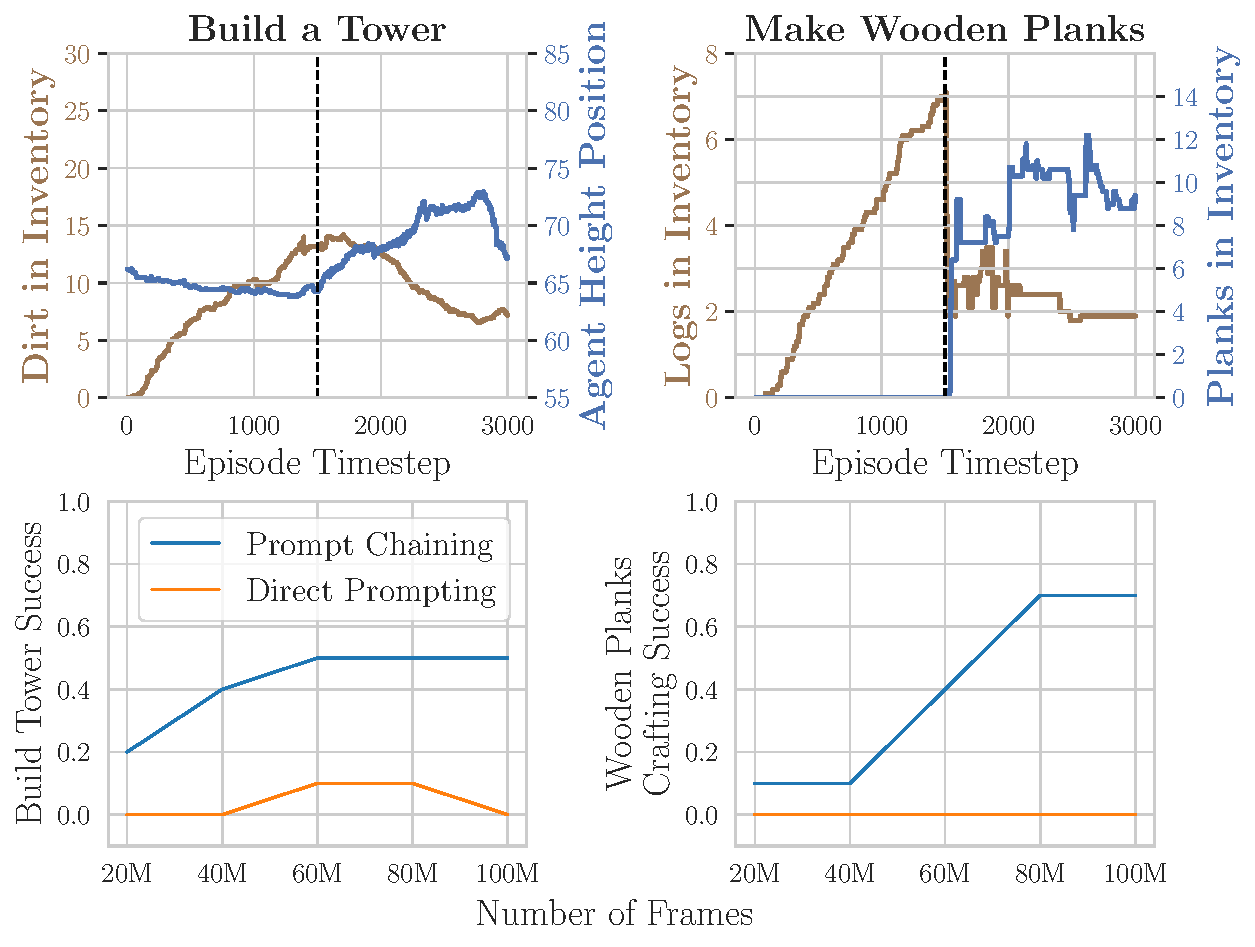
\includegraphics[width=0.985\textwidth]{figures/4.2_chaining_success_and_episode.pdf}
        \label{fig:chaining_eps}
        % \caption{Prompt Chaining}
    \end{subfigure}
    \begin{subfigure}{0.48\textwidth}
        \centering
            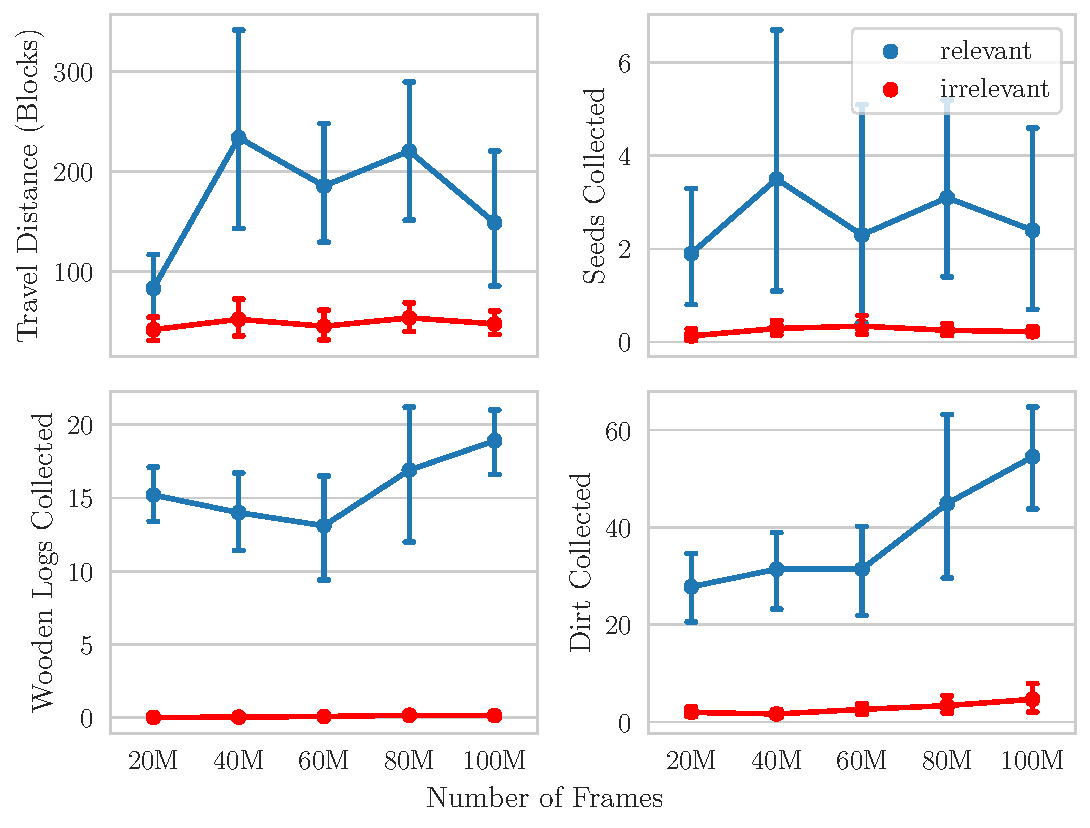
\includegraphics[width=0.96\textwidth]{figures/4.2_scaling_programmatic_arxiv.pdf}
            \label{scaling_prog}
            % \caption{Scaling across number of frames}
    \end{subfigure}
    \caption{\textbf{Top left}: By sequentially chaining visual prompts like ``get dirt'' and ``build a tower'', \agentname{} successfully gathers dirt and then uses this dirt to build a tower. The prompts switch at the dotted vertical line. \textbf{Bottom left}: The success rates of the chained prompts improve steadily as we train \agentname{} on more data. \textbf{Right}: The performance of \agentname{} on different tasks scales in different ways when conditioning on a relevant visual prompt for the metric versus other irrelevant visual prompts (e.g., the break wood prompt is the relevant prompt for the ``Wooden Logs Collected'' metric, while the other prompts are ``irrelevant''). For instance, in the wood-collection and dirt-collection tasks, performance starts increasing after training on 60M frames of gameplay. See \autoref{fig:apdx_visual_goals} for sample frames from each visual prompt.}
    \label{fig:chaining}
    \vspace{-1em}
\end{figure}

\subsection{Scaling}
\label{sec:scaling}

Recent works in language modeling have found that scaling up pretraining FLOPs, by training on more data or by training a model with more parameters, can improve performance on downstream tasks \cite{scalinglaws, bigbench, emergent}. In certain cases when measuring performance with metrics such as exact-match \citep{emergent_mirage}, performance improvement may appear to be ``emergent'' \citep{emergent}, appearing suddenly as the model is trained with more compute. Here, we aim to gain a basic understanding of how the performance of \agentname{} on various tasks scales by training with more data (learning rate schedule is chosen appropriately). 

To assess performance gain, we isolate the performance of the policy from the prior, measuring performance of the agent on programmatic tasks (travel distance, seeds, logs, dirt) with visual goals. Due to compute constraints, we chose to use the 2x VPT model, which has 248M parameters. We found that both seed collection and travel distance did not improve significantly past 20M frames. From inspecting gameplay, we suspect that travel distance is a relatively easy task since it is close to VPT's default behavior of running around and exploring. For seed collection, performance remains suboptimal, suggesting that further scaling may be beneficial. This hypothesis is supported by the observation that performance on log and dirt collection remained roughly level until 60M frames when it began to rapidly improve. \autoref{fig:chaining} shows the scaling curves for \agentname{} on each programmatic task when conditioning on relevant vs. irrelevant visual prompts for that task. Since we do not observe regression on any tasks as we train the model with more compute, we expect the model to continue to perform better as we train larger models on larger datasets.

We also evaluated the scaling properties of \agentname{} for our multi-step tasks with and without prompt chaining. Without prompt chaining, the tasks remain challenging for \agentname{} throughout training. However, we note that after 60M frames, \agentname{} sometimes gathers wooden logs and then builds a small tower when directly prompted to build a tower. This is likely because our visual prompt for tower building shows a video of a tower being built out of wooden logs. With prompt chaining, the performance of \agentname{} steadily increases with more data. We conjecture that this is because the success of a chained prompt requires the success of each element in the chain. Since different abilities emerge at different scales, one would expect chained prompts to steadily get more reliable as these subgoals become more reliably completed. In the case of crafting wooden planks, we note that crafting is one such task that gets significantly more reliable as the agent is trained on more data. \autoref{fig:chaining} shows the scaling curves for \agentname{} on the prompt chaining tasks.

In summary, we see evidence of tasks that do not require much data for \agentname{} to learn, tasks that steadily get more reliable as the agent is trained longer, and tasks where capability suddenly spikes after the agent reaches some threshold. Put together, this suggests that further scaling would likely significantly improve the agent, although we leave the task of predicting exactly how much performance there is to gain to future studies.

\subsection{What Matters for Downstream Performance?}

\paragraph*{Pretraining} \citet{baker2022vpt} finds that by pretraining a behavioral prior with imitation learning on internet-scale datasets for Minecraft, the learned policy can be effectively finetuned to accomplish tasks that are impossible without pretraining. In this section, we demonstrate that pretraining is also massively beneficial for instruction-tuning in Minecraft. We hypothesize that due to the strong performance of \agentname{} and the relatively small amount of compute ($\approx 1\%$ additional compute) used for instruction finetuning, most of the capabilities of our agent come from the pretraining rather than the finetuning. To test this hypothesis, we finetune several varients of \agentname{} from various pretrained weights: \texttt{foundation-2x}, \texttt{bc-early-game-2x}, \texttt{rl-from-foundation-2x}, and with randomly initialized weights. In this experiment, each model was finetuned on 100M frames.

\autoref{fig:pretraining_cond_scale} shows the performance of these models on our programmatic tasks with visual goals. Note that while an agent trained on our dataset from scratch can accomplish basic tasks like dirt collection fairly well, it is unable to find and chop down trees, in contrast to the pretrained agents. This demonstrates that the abilities present in the agent due to pretraining are successfully transferred to the finetuned agent. Out of all the pretrained weights we tried, we noticed that \texttt{rl-from-foundation-2x} performed the best, having qualitatively better performance at tasks like crafting and chopping down trees. Indeed, \autoref{fig:pretraining_cond_scale} shows that this model has strong performance, likely due to the massive amount of compute it was trained with during its RL training \citep{baker2022vpt}.

\paragraph*{Classifier-Free Guidance} \label{par:cfg} \citet{baker2022vpt} observed that when conditioning the agent on text, it tended to ignore its instruction and instead perform the prior behavior learned during pretraining. As discussed in \Cref{sec:inference}, classifier-free guidance \citep{cfg} gives a knob for trading off between goal-conditioned and prior behaviors. \autoref{fig:pretraining_cond_scale} shows the effect of this parameter $\lambda$ on the log and dirt collection tasks. The performance of the agent reaches its maximum around $\lambda = 5.0$ to $\lambda = 7.0$, after which it starts to drop off. These results demonstrate the importance of classifier-free guidance, which improves the performance of \agentname{} by orders of magnitude.

\begin{figure}
    \centering
    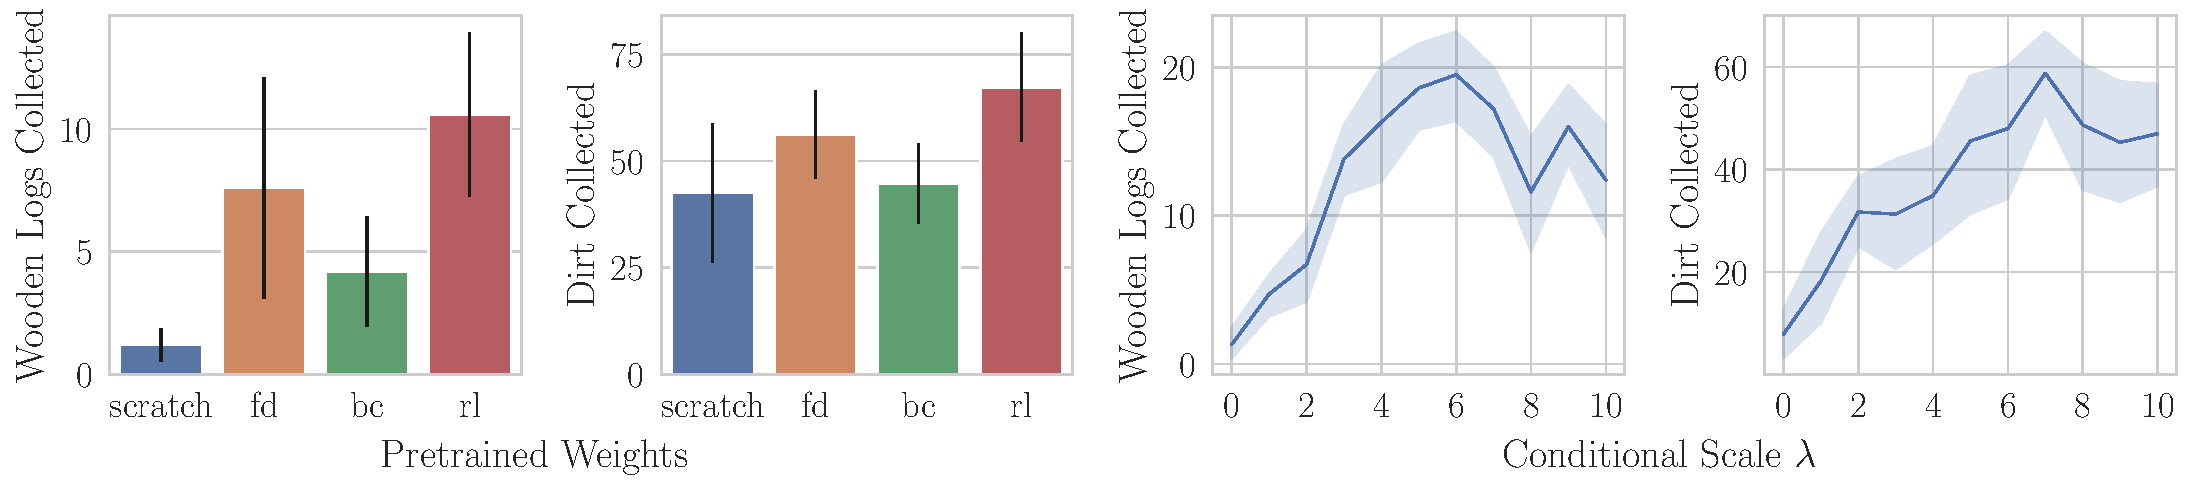
\includegraphics[width=\textwidth]{figures/4.4_pretrained_and_cond_scale_value.pdf}
    \caption{\textbf{Left:} We trained \agentname{} on 100M frames starting from four different pretrained weights: random initialization (scratch), \texttt{foundation-2x} (fd), \texttt{bc-early-game-2x} (bc), and \texttt{rl-from-foundation-2x} (rl). The \texttt{rl-from-foundation-2x} agent is generally the most performant after fine-tuning. Using pretrained weights performs better than training from scratch, especially for more complicated tasks like collecting wood. \textbf{Right:} By using classifier-free guidance \citep{cfg}, \agentname{} collects \(7.5 \times\) more dirt and \(15 \times\) more wood than when $\lambda = 0$ (no guidance). See \autoref{fig:full_cond_scale_exps} in the Appendix for similar results with other  programmatic tasks.}
    \label{fig:pretraining_cond_scale}
    \vspace{0.75em}
\end{figure}

\paragraph*{Prompt Engineering} Prompt engineering as a discipline has rapidly emerged over the last year due to the observation that the quality of the output of text-to-X models can dramatically change depending on the prompt \citep{zhou2023large}. For example, \autoref{table:prompt-evolution} in the appendix shows how a prompt for Stable Diffusion \citep{rombach2022ldm} might be written. By listing out the various attributes of the image such as visual medium, style, and the phrase ``trending on ArtStation'', the user is able to get a higher quality image \citep{sdprompts, prompts}. In this section, we explore how this same style of prompt engineering can improve the performance of \agentname. \autoref{fig:prompt_performance} shows how a simple prompt of ``get dirt'' might be changed in order to more accurately specify the type of behavior that is desired. Just like in image generation models, the performance of \agentname{} significantly improves by modifying the prompt in this fashion. By changing to more complicated prompts, \agentname{} is able to collect \(1.6\times \) more wood, \(2\times \) more dirt, and \(3.3\times \) more~seeds.

\begin{figure}
    \centering
    \begin{tabular}{ll}
\toprule
Prompt & Dirt Collected \\
\midrule
``break a flower'' & 0.7 (-0.2, 1.6) \\
``collect seeds'' & 2.7 (0.9, 4.5) \\
``dig as far as possible'' & 3.9 (2.8, 5.0) \\
``get dirt'' & 9.2 (5.7, 12.7) \\
``get dirt, dig hole, dig dirt, gather a ton of dirt, collect dirt'' & \textbf{26.7 (19.9, 33.5)} \\
\bottomrule
\end{tabular}
    \vspace{0.25em}
    \caption{Similar to text-to-image generation, switching to a longer, more specific prompt dramatically improves the performance of \agentname{}. Values in parentheses are 95\% confidence intervals.}
    \label{fig:prompt_performance}
\end{figure}

